\documentclass[10pt,a4paper]{article}
\usepackage[utf8]{inputenc}
\usepackage{amsmath}
\usepackage{amsfonts}
\usepackage{amssymb}
\usepackage{graphicx}
\usepackage{todo}
\usepackage[left=2cm]{geometry}
\author{Christoph Robbert 6577945, Peter Stilow 6500440}
\title{Protokoll 0}
\begin{document}
\maketitle
 
\section{Aufgabe 1}
Nach einem Login auf den Rechner \texttt{cultofthedeadcow.seclab.uni-paderborn.de/192.26.175.11} sah man an der Ausgabe von \texttt{ifconfig}, dass sich dieser Rechner im Subnetz \texttt{192.26.175.0/26} befand.
Ein Anschließender Pingscan mittels \texttt{nmap -sP 192.26.175.0/26} zeigte, dass die Hosts aus Figure \ref{0_netlayout} in diesem Subnetz erreichbar sind.
Außerdem zeigte ein anschließender Portscan( \texttt{nmap -sT -sV} die folgenden offenen Ports:
\begin{figure}
	\label{0_netlayout}
	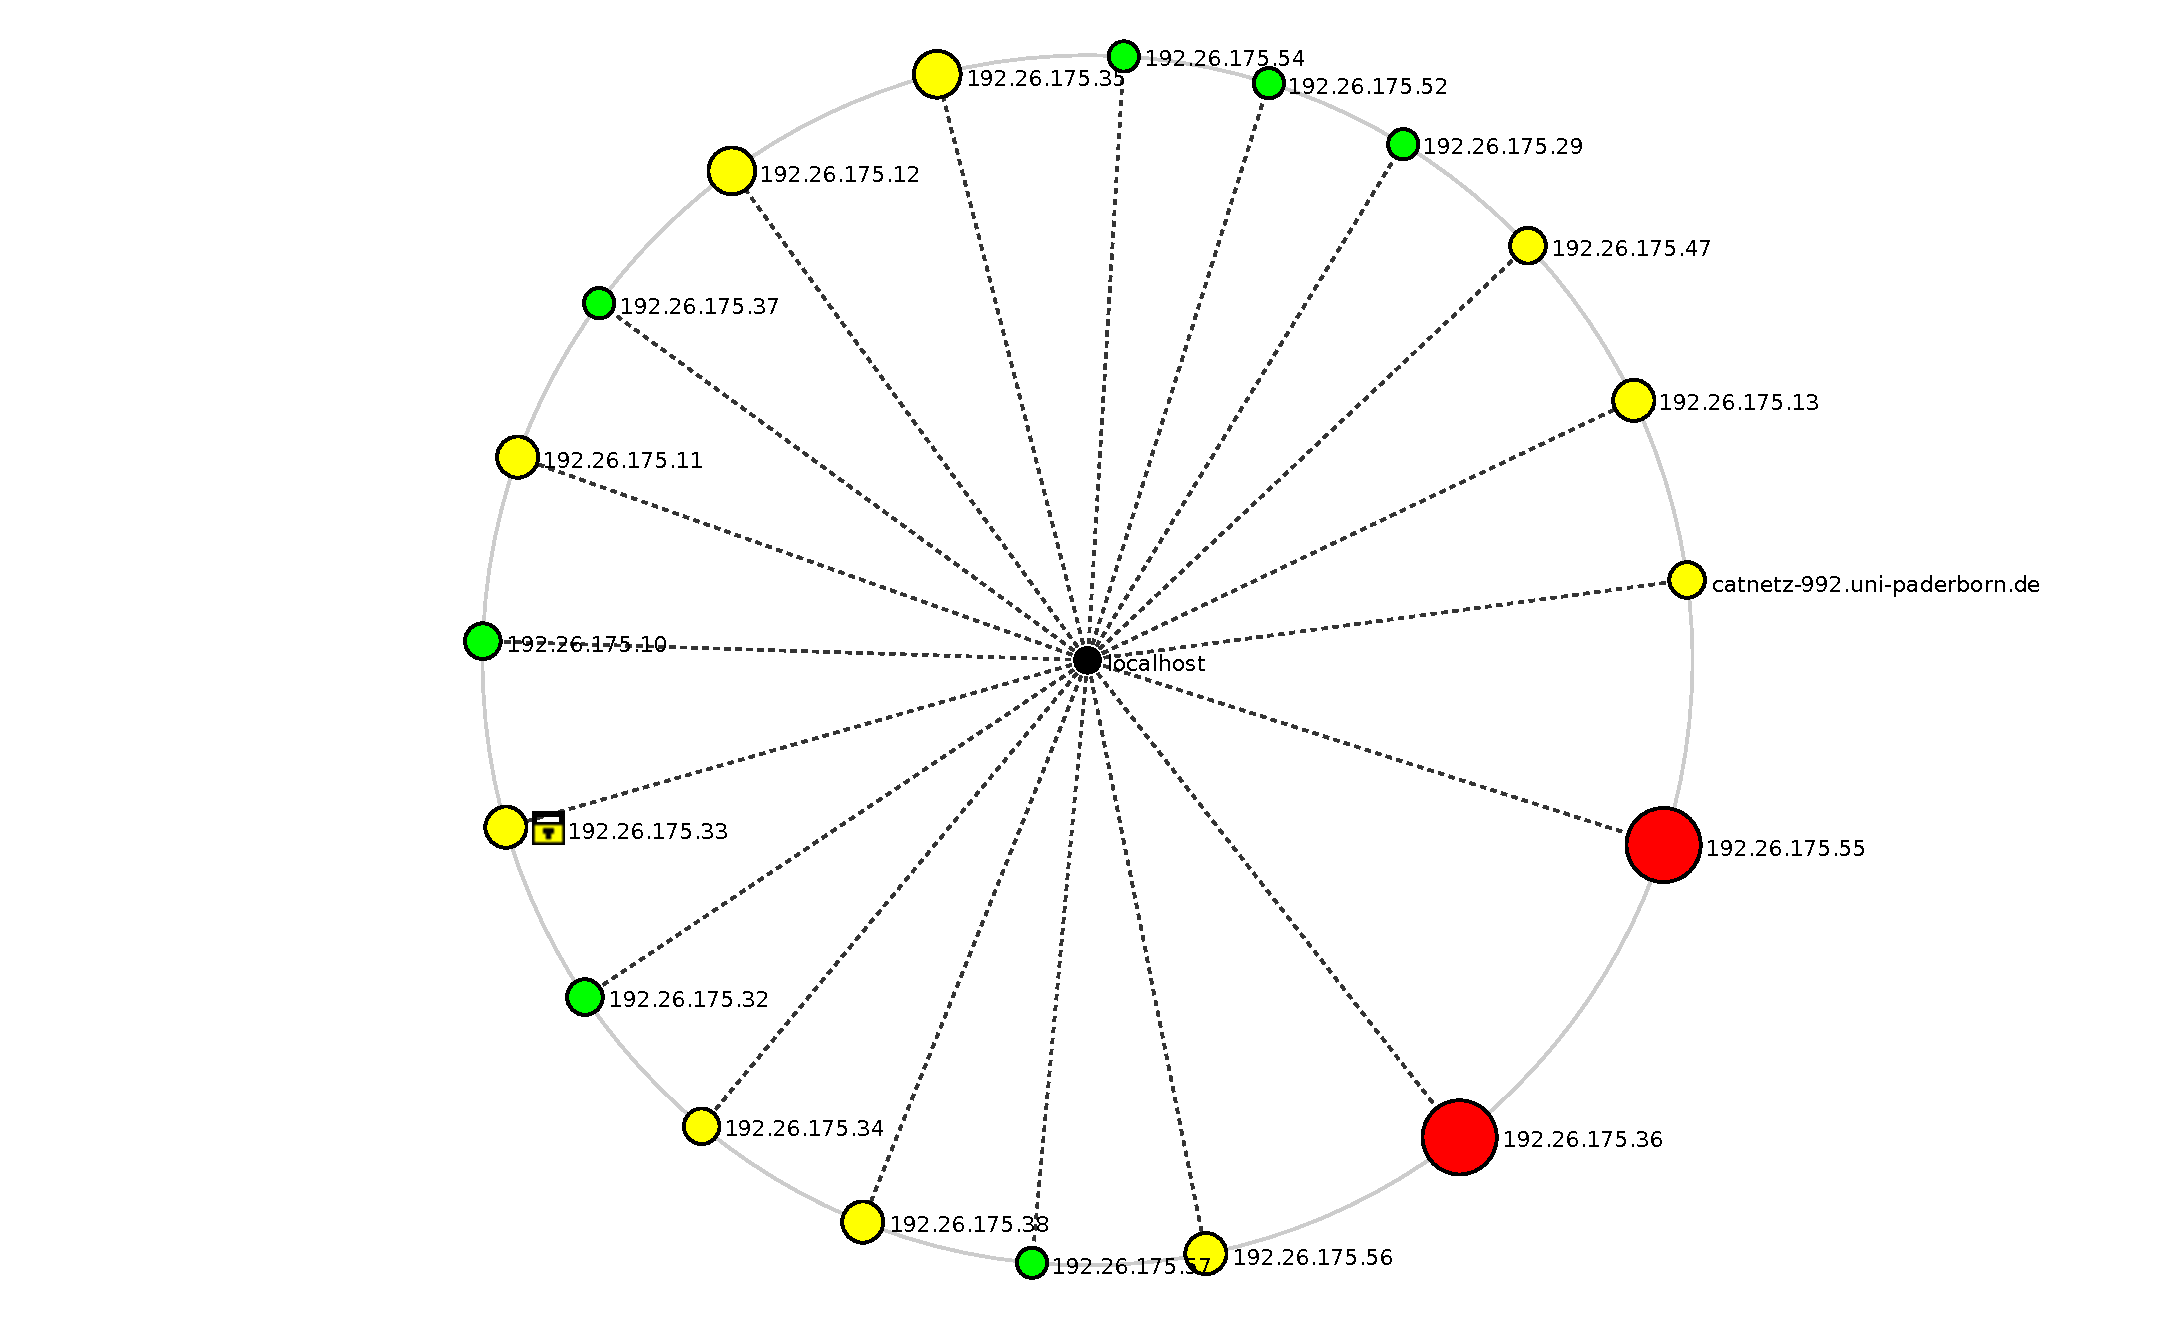
\includegraphics[scale=0.4]{figures/0_netlayout.pdf}
	\caption{Struktur des Netzes im Security Lab.}
\end{figure}

\begin{description}
	\item[catnetz-992.uni-paderborn.de (192.26.175.1)] Ergebnisse Portscan:
	\begin{verbatim}
22/tcp  open  ssh      Cisco SSH 1.25 (protocol 1.99)
80/tcp  open  http     Cisco IOS administrative httpd
443/tcp open  ssl/http Cisco IOS administrative httpd
Service Info: OS: IOS
	\end{verbatim}
Aus den Angaben des Portscan lässt sich schließen, dass es sich um einen Cisco Router handelt bei diesem Host. Da die Automatische Dienstanalyse von \texttt{nmap} sowohl bei den Diensten Cisco Dienste identifiziert als auch bei der Service Info das Routerbetriebssystem IOS. 

	\item[192.26.175.10] Ergebnisse Portscan:
	\begin{verbatim}
22/tcp  open  ssh     OpenSSH 5.9p1 Debian 5ubuntu1 (protocol 2.0)
111/tcp open  rpcbind
Service Info: OS: Linux
	\end{verbatim}
Bei diesem Host wird es sich um einen Ubuntu 12.04 Rechner handeln. Dies schließen wir aus dem Versionsstring '5ubuntu1', da diese Version des openssh Servers nur in Ubuntu 12.04 verwendet wurde. Außer dem ssh und dem rpcbind Dienst wurde kein Dienst auf diesem Server identifiziert.

	\item[cultofthedeadcow.seclab.uni-paderborn.de (192.26.175.11)] Ergebnisse Portscan:
	\begin{verbatim}
22/tcp   open  ssh           OpenSSH 5.9p1 Debian 5ubuntu1.1 (protocol 2.0)
111/tcp  open  rpcbind
3389/tcp open  microsoft-rdp xrdp
8080/tcp open  http          Apache Tomcat/Coyote JSP engine 1.1
Service Info: OS: Linux
	\end{verbatim}
Dieser Rechner ist ein Ubuntu 12.04.3 Rechner. Da Zugang zu diesem Rechner per SSH besteht kann man via \texttt{vim /etc/issue} diese Versionbezeichung eindeutig bestimmen. Neben dem schon bekannten SSH Dienst läuft auch ein rpcbind Dienst, ein Apache Tomcat Anwendungsserver und der microsoft-rdp Dienst für RemoteDesktopverbindungen.

	\item[192.26.175.12] Ergebnisse Portscan:
	\begin{verbatim}
22/tcp   open  ssh           OpenSSH 5.9p1 Debian 5ubuntu1.1 (protocol 2.0)
111/tcp  open  rpcbind
3389/tcp open  microsoft-rdp xrdp
5910/tcp open  vnc           VNC (protocol 3.3; Locked out)
Service Info: OS: Linux
	\end{verbatim}
Dieser Rechner scheint auch ein Ubuntu 12.04 Rechner zu sein. Neben dem openssh Server und dem rpcbind Dienst scheint auch ein microsoft-rdp Dienst und ein VNC Dienst für Remotelogins aktiv zu sein.

\item[192.26.175.13]
Der Portscan brachte dieselben Ergebnisse wie beim Rechner mit der IP 192.26.175.11

\item[192.26.175.14]
Der Portscan brachte dieselben Ergebnisse wie beim Rechner mit der IP 192.26.175.12

\item[192.26.175.29] Ergebnisse Portscan:
	\begin{verbatim}
139/tcp open  netbios-ssn
137/udp open|filtered netbios-ns
138/udp open|filtered netbios-dgm
	\end{verbatim}
Da hier der netbios Dienst läuft, schließen wir, dass es sich um einen Windows Rechner handelt. Die genaue Version ist Aufgrund der Portscans nicht zu ermitteln.

\item[192.26.175.32] Ergebnisse Portscan:
\begin{verbatim}
22/tcp open  ssh     OpenSSH 5.8p2_hpn13v11 (FreeBSD 20110503; protocol 2.0)
25/tcp open  smtp
\end{verbatim}
Bei diesem Rechner wird es sich laut der verwendeten OpenSSH Serverversion um einen FreeBSD Rechner handeln. Neben dem OpenSSH Server läuft auch ein smtp Server(E-Mail annehmender Server). 

\item[192.26.175.33] Ergebnisse Portscan:
\begin{verbatim}
13/tcp   open     daytime
22/tcp   open     ssh     OpenSSH 5.9 (protocol 2.0)
37/tcp   open     time    (32 bits)
113/tcp  open     ident
6000/tcp filtered X11
6001/tcp filtered X11:1
6002/tcp filtered X11:2
6003/tcp filtered X11:3
6004/tcp filtered X11:4
6005/tcp filtered X11:5
6006/tcp filtered X11:6
6007/tcp filtered X11:7
6009/tcp filtered X11:9
Service Info: OS: Unix
\end{verbatim}
Dieser Rechner besitzt auch ein Unix System, scheinbar aber nicht um die Ubuntu version 12.04,
da hier OpenSSH anders ist. Außerdem gibt es hier auch andere offene Ports, z.B. für daytime und time.

\item[192.26.175.34] Ergebnisse Portscan:
\begin{verbatim}
135/tcp open  msrpc        Microsoft Windows RPC
139/tcp open  netbios-ssn
445/tcp open  microsoft-ds Microsoft Windows XP microsoft-ds
Service Info: OS: Windows; CPE: cpe:/o:microsoft:windows
\end{verbatim}
Auf diesem PC läuft Windows XP, wie man an microsoft-ds erkennen kann.

\item[192.26.175.35] Ergebnisse Portscan:
\begin{verbatim}
21/tcp   open  ftp     ProFTPD 1.3.4a
22/tcp   open  ssh     OpenSSH 5.9p1 Debian 4 (protocol 2.0)
80/tcp   open  http    Apache httpd 2.2.22 ((Debian))
111/tcp  open  rpcbind 2-4 (RPC #100000)
548/tcp  open  afp     Netatalk 2.2.2 (name: flgd0d1741e939d8fc51e0dae50ff39; protocol 3.3)
3306/tcp open  mysql   MySQL 5.1.61-2
Service Info: OSs: Unix, Linux; CPE: cpe:/o:linux:linux_kernel
\end{verbatim}
Bei diesem Rechner handelt es sich wieder um eine Ubuntu Installation. Zusätzlich zu den vorherigen laufen auf diesem hier allerdings ein ftp- sowie ein MySQL-Server. Der Name dieses Rechners (als UTF-8) ist zusätzlich ein flag aus der nächsten Aufgabe.

\item[192.26.175.36] Ergebnisse Portscan:
\begin{verbatim}
1/tcp     open  tcpwrapped
22/tcp    open  ssh        OpenSSH 5.9p1 Debian 4 (protocol 2.0)
79/tcp    open  tcpwrapped
111/tcp   open  rpcbind    2-4 (RPC #100000)
119/tcp   open  tcpwrapped
143/tcp   open  tcpwrapped
1080/tcp  open  tcpwrapped
1524/tcp  open  tcpwrapped
2000/tcp  open  tcpwrapped
6667/tcp  open  tcpwrapped
12345/tcp open  tcpwrapped
31337/tcp open  tcpwrapped
32771/tcp open  tcpwrapped
32772/tcp open  tcpwrapped
32773/tcp open  tcpwrapped
32774/tcp open  tcpwrapped
Service Info: OS: Linux; CPE: cpe:/o:linux:linux_kernel
\end{verbatim}
Auch dieser PC besitzt wieder die gleiche Ubuntu Version und besitzt wieder den ssh Zugang. Zusätzlich besitzt der Computer scheinbar eine Firewall, die die meisten offenen Ports vor Unbefugten zugriffen schützt.

\item[192.26.175.37] Ergebnisse Portscan:
\begin{verbatim}
22/tcp open  ssh     OpenSSH 6.3 (protocol 2.0)
\end{verbatim}
Über diesen Computer gibt es nicht viele Informationen, außer, dass es einen ssh Zugang gibt.

\item[192.26.175.38] Ergebnisse Portscan:
\begin{verbatim}
21/tcp  open  ftp         vsftpd 3.0.2
22/tcp  open  ssh         OpenSSH 6.3 (protocol 2.0)
139/tcp open  netbios-ssn Samba smbd 3.X (workgroup: ARCH)
445/tcp open  netbios-ssn Samba smbd 3.X (workgroup: ARCH)
Service Info: OS: Unix
\end{verbatim}
Auf diesem Rechner befindet sich ein Unix System (Arch-Linux?), der sowohl einen ssh Zugang bietet, als auch einen ftp Server, sowie eine Windows-Netzwerk Umgebung durch den Samba Service.

\item[192.26.175.47] Ergebnisse Portscan:
\begin{verbatim}
22/tcp open  ssh     Dropbear sshd 0.53.1 (protocol 2.0)
53/tcp open  domain  dnsmasq 2.55
80/tcp open  http    LuCI Lua http config
Service Info: OS: Linux; CPE: cpe:/o:linux:linux_kernel
\end{verbatim}
Auch auf diesem Rechner läuft ein Unix System, welches zusätzlich zum ssh Zugang auch einen http Server bereit stellt.


\item[192.26.175.55] Ergebnisse Portscan:
\begin{verbatim}
7/tcp    open  echo
9/tcp    open  discard?
13/tcp   open  daytime       Microsoft Windows USA daytime
17/tcp   open  qotd          Windows qotd (English)
19/tcp   open  chargen
21/tcp   open  ftp           Microsoft ftpd
25/tcp   open  smtp          Microsoft ESMTP 6.0.3790.3959
135/tcp  open  msrpc         Microsoft Windows RPC
139/tcp  open  netbios-ssn
445/tcp  open  microsoft-ds  Microsoft Windows 2003 or 2008 microsoft-ds
548/tcp  open  afp?
1025/tcp open  msrpc         Microsoft Windows RPC
1028/tcp open  msrpc         Microsoft Windows RPC
1029/tcp open  msrpc         Microsoft Windows RPC
1030/tcp open  msrpc         Microsoft Windows RPC
3389/tcp open  ms-wbt-server Microsoft Terminal Service
8099/tcp open  http          Microsoft IIS httpd 6.0
Service Info: Host: w2k3; OS: Windows; CPE: cpe:/o:microsoft:windows
\end{verbatim}
Auf diesem Computer läuft das MS Windows 2003 Betriebssystem. Er besitzt sowohl einen ftp- und einen http-Server und bietet den normalen Windows Netzwerk Dienst.

\item[192.26.175.56] Ergebnisse Portscan:
\begin{verbatim}
22/tcp  open  ssh        Dropbear sshd 0.53.1 (protocol 2.0)
53/tcp  open  domain     dnsmasq 2.55
80/tcp  open  http?
443/tcp open  ssl/https?
Service Info: OS: Linux; CPE: cpe:/o:linux:linux_kernel
\end{verbatim}
Auf diesem Rechner läuft wieder ein Linux, ähnlich zu dem 192.26.175.47. Zusätzlich zum http Server gibt es hier auch einen https Server.


\end{description}

\section{Aufgabe 2}
\begin{description}
	\item[flgbab8e275f92ee6cf9fd48333dfeb0b85] Beim Aufstellen der Stützen unter der Tastatur fiel dieser Hardwareflag auf. 
	\item[flgbb315509cf9c5caac09624d258c3d95d] Beim einloggen via \texttt{ssh} auf den Rechner \texttt{192.26.175.11} und anschließendem "orientieren" via \texttt{ls} fiel auf, dass ein Windowsbatch mit dem Namen \texttt{runme.bat} auf einem Linuxsystem erstellt wurde. Um zu schauen was es damit aufsich hat, begutachteten wir den Inhalt des Skriptes mittels \texttt{vim}. Das Skript gibt via \texttt{echo} den String dieses Flags aus.
	Außerdem fanden wir dieses Flag auf dem FTP Server auf dem Rechner \texttt{192.26.175.38} in der Datei \\ \texttt{/follow/the/white/rabbit/runme.bat}
	\item[flg58594831dfbe63560f940365d517fa68] Zum finden dieses Flags haben wir mit Wireshark im Capture Mode einfach alle Packete im Netzwerk abgefangen. Dabei fiel dieses Flag in einen UDP Packet vom Rechner 192.26.175.36 zum Rechner 192.26.175.63 auf.
	\item[flg8e7fa2f4b3e3390175badcc38141bd1f] Auf dem Rechner \texttt{192.26.175.35} läuft ein FTP-Server. Beim Durchsuchen der Inhalte fiel eine Datei auf, in der der Benutzer Bernd dazu aufgefordert wurde ein Passwort für sein MySQL Account zu setzen. Da auf demselben Rechner ein MySQL Server lief, loggten wir uns als Benutzer \texttt{bernd} auf diesem MySQL Server ein. In der Datenbank \texttt{bernd} fanden wir die Tabelle \texttt{hier\_gibts\_aktuelle\_flags}. Ein \texttt{select * from hier\_gibts\_aktuelle\_flags;} brachte das obengenannte Flag zu Tage.
	\item[flg0607547c0d12497a21ab8a0b53dd5bed] Auf dem Rechner \texttt{192.26.175.35} läuft auch ein HTTP-Server. Beim Aufrufen der URL \texttt{http://192.26.175.35} fanden wir im HTML-Quelltext der angezeigten Website dieses Flag. Es war im Webbrowser nicht zu sehen, da es auskommentiert wurde im HTML Quellcode.
	\item[flgd0d1741e939d8fc51e0dae50ff39bed4] Beim Scannen des Rechners \texttt{192.26.175.35} mit dem nmap Kommando \texttt{nmap -T4 -A -v 192.26.175.35} viel als UFT8 Servername im Dienst Netatalk dieses Flag auf.
	\item[flg9fa80db0f34a75d1f474f29e8ed8f1ac] In der SMB Freigabe \texttt{smb://arch/dontlookhere/} fanden wir das Bild \texttt{SMBFLAG.png}. Der Inhalt des Bildes enthielt die oben genannte Flag.
	\item[flgc905381d9e34b1efd02594423806e1d7] Beim Beobachten des Netzwerkverkehrs in Wireshark viel uns ein Packet von \texttt{192.26.175.38} nach \texttt{192.26.175.63} auf in dem stand \texttt{bernd@192.26.175.37} gefolgt von zwei Packeten die einen RSA Private Key enthielten. Nachdem wir uns mit dem Private Key per \texttt{ssh bernd@192.26.175.37} einloggten, erschien der Key auf der Kommandozeile.
\end{description}

\end{document}